% \vspace{-1em}
\section{Proposed Commonsense Reasoning Benchmark}
\label{sec:benchmark}
% \vspace{-1em}
% \begin{table*}[t]
    \caption{Different reasoning templates of the statements that we uncovered, presumably reflecting how humans logically reason. $\wedge$, $\neg$, $\coloneq$ indicate logical and, negation, and implication, respectively. $\textAction_h$ is an action that is hidden in the main utterance and $\textAction(\textState)$ indicates performing the $\textAction$ when the $\textState$ holds.}
    \label{tab:logic_templates}
\centering
\resizebox{0.9\textwidth}{!}{%
    \begin{tabular}{llc}
        \toprule 
        \bf{Logic template} & \textbf{Example} & \bf{Count} \\
        \midrule
        1. \thead[l]{\blueTemplate{$(\neg(\text{\textGoal}) \coloneq \text{\textState}) \wedge$} \\ \blueTemplate{$(\text{\textGoal} \coloneq \text{\textAction}(\text{\textState}))$}} & \thead[l]{If it snows tonight \\ then wake me up early \\ because I want to arrive to work on time} & 65 \\
        % &  &\\
        2. \thead[l]{\orangeTemplate{$(\text{\textGoal} \coloneq \text{\textAction}(\text{\textState})) \wedge$} \\ \orangeTemplate{$(\neg(\text{\textGoal}) \coloneq \neg(\text{\textAction}(\text{\textState})))$}} & \thead[l]{If I am walking to a meeting \\ then remind me who else is there \\ because I want to be prepared for the meeting} & 50 \\
        % & &\\
        3. \thead[l]{\greenTemplate{$(\text{\textGoal} \coloneq \text{\textAction}_h) \wedge$} \\ \greenTemplate{$(\text{\textAction}_h \coloneq \text{\textAction}(\text{\textState}))$}} & \thead[l]{If we are approaching Fall \\ then remind me to buy flower bulbs \\ because I want to make sure I have a pretty Spring garden.} & 17 \\
        % & &\\
        4. \thead[l]{\purpleTemplate{$(\text{\textGoal} \coloneq \text{\textState}) \wedge$} \\  \purpleTemplate{$(\neg(\text{\textGoal}) \coloneq \text{\textAction}(\text{\textState}))$}}
        & \thead[l]{If I am at the grocery store but I have a trip coming up in the next week \\ then remind me not to buy perishables \\ because they will go bad while I am away} & 5 \\
        % & & \\
        % 5. \thead[l]{\pinkTemplate{$(\text{\textState} \coloneq \text{\textAction}) \wedge$} \\ \pinkTemplate{$(\text{\textAction} \coloneq \text{\textGoal})$}} & \thead[l]{If I schedule an appointment that overlaps with another appointment \\ then notify me immediately \\ because I want to notify my colleagues of the conflict.} & 1 \\
        % & & \\
        5. \redTemplate{other} & \thead[l]{If tomorrow is a holiday \\ then ask me if I want to disable or change my alarms \\ because I don't want to wake up early if I don't need to go to work early.}  &23 \\
        \bottomrule
    \end{tabular}
    }
\end{table*}
% \amoscomment{I'm missing some opening sentence or two before you dive into technical details and notation. at least something like: In this work we assume that the input statements to the system ...}
% \vspace{-1em}
The benchmark task that we propose in this work is that of uncovering hidden \emph{commonsense presumptions} given commands that follow the general format ``if $\langle$state holds$\rangle$ then $\langle$perform action$\rangle$ because $\langle$I want to achieve goal$\rangle$''. 
We refer to these as if-then-because commands. 
% Formally, the commands
We refer to the \emph{if}-clause %Amos: shouldn't it be the if-clause or some other word (not "statement", because the entire if-then-because is called a statement.) Same goes for the "because" statement. % Forough: addressed
as the \textState, the \emph{then}-clause as the \textAction and the \emph{because}-clause as the \textGoal. 
% Please note that the because-clause is included to help disambiguate the underlying intent of each statement (refer to the example in the Introduction) without which it might be impossible to correctly uncover the unspoken commonsense presumptions. %Amos: I think that the previous sentence is redundant, especially if we don't have enough room. Forough: Thanks, removed
These natural language commands were collected from a pool of human subjects (more details in the Appendix). 
% and are free-form natural language sentences. 
The data is annotated with unspoken commonsense presumptions by a team of annotators. Tab.~\ref{tab:statement_stats} shows the statistics of the data and annotated examples from the data.
% (see Tab.~\ref{tab:data_examples} in the Appendix for examples of the annotated data).
% \section{Datasets}
We collected two sets of if-then-because commands.
% from human subjects (please refer to the Appendix for a more statistics). 
The first set contains 83 commands targeted at a \textState that can be observed by a computer/mobile phone (%which is
e.g. checking emails, calendar, maps, alarms, and weather). The second set contains 77 commands whose \textState is about day-to-day events and activities. 81\% of the commands over both sets qualify as ``if $\langle \text{\,\textState} \rangle $ then $\langle \text{\,\textAction} \rangle $ because $\langle \text{\,\textGoal} \rangle $''. The remaining 19\% differ in the categorization of the \textit{because}-clause (see Tab.~\ref{tab:statement_stats}); common alternate clause types included anti-goals (``...because I don't want to be late''), modifications of the state or action (``... because it will be difficult to find an Uber''), or conjunctions including at least one non-goal type. Note that we did not instruct the subjects to give us data from these categories, rather we uncovered them after data collection. 
% We selected only statements with goal-type because clauses for the work to follow but all the statements are released with the data. 
% \tmcomment{I suggest delete the next sentence}\facomment{removed} We would like to add that these commands are not to be used for training purposes, and are instead a benchmark task carefully designed and annotated to test machine common sense, defined as the ability of inferring hidden commonsense presumptions in if-then-because commands. 
% Note that
Also, commonsense benchmarks such as the Winograd Schema Challenge \cite{levesque2012winograd} included a similar number of examples (100) when first introduced \cite{kocijan2020review}.% and was scaled up very recently \cite{sakaguchi2019winogrande}.

Lastly, % after collecting the data we discovered that 
the if-then-because commands given by humans can be categorized into several different logic templates. 
% This is in contrary to the belief in the reasoning community that a single reasoning strategy could solve all reasoning problems, at least in a single benchmark. 
The discovered logic templates are given in Table \ref{tab:logic_templates} in the Appendix \footnote{The appendix is available at https://arxiv.org/abs/2006.10022}. Our neuro-symbolic theorem prover uses a general reasoning strategy that can address all reasoning templates. However, in an extended discussion in the Appendix, we explain how a reasoning system, including ours, could potentially benefit from these logic templates.

% \tmcomment{we don't really mean "when generating" commands do we in the next sentence?  Don't we mean that humans use different strategies to "reason about them"?   Also, doesn't it sound incorrect to claim that we know how humans reason?  Maybe delete this next paragraph except keep only the final sentence? } \facomment{ I changed it to the above, paragraph. (by the final sentence do you mean the sentence in line 12 of the latex source? or line 15 of the latex source?) Does it look good now?} After collecting the statements, we noticed that humans have different reasoning strategies when generating if-then-because commands. This is in contrary to the belief in the reasoning community that a single reasoning strategy could solve all reasoning problems, at least in a single benchmark.
% We believe this is a valuable finding because it indicates that researchers should perhaps consider these different reasoning strategies 
% shed some light on the different aspects of  what to consider when addressing reasoning problems. 
% The logic reasoning templates we discovered in the data are in Table \ref{tab:logic_templates} in the Appendix.
\vspace{-0.5em}
% We have further categorized the collected statements into four different logic templates listed in Tab.~\ref{tab:statement_stats}, right sub-table. The logic templates reflect how humans reason about if-then-because statements. 
\begin{figure*}[t!]
\centering
\tikzset{%
process/.style  = {rectangle, minimum width=1cm, minimum height=1cm, align=flush center, draw=black, inner sep=0.2cm},
decision/.style = {diamond, minimum width=1cm, minimum height=1cm, align=flush center, draw=black, inner sep=0cm},
resource/.style = {shape=rounded rectangle, minimum width=1cm, minimum height=1cm, align=flush center, draw=black},
stop/.style     = {rectangle, minimum width=1cm, minimum height=1cm, align=flush center, draw=black, double, thick},
waypoint/.style = {coordinate}
}
\newcommand{\cbox}[2]{\parbox{#1}{\centering
#2}}
\newcommand{\mrule}[1]{\rule[0.8ex]{#1}{0.4pt}}
\resizebox{0.85\textwidth}{!}{%
\begin{tikzpicture}[
thick,
>/.tip=Latex,
loose/.style={inner sep 0.7em}]
\draw
	node at (0,0) [font=\large] (statement) {input: If $\langle$\textState$\rangle$ then $\langle$\textAction$\rangle$ because $\langle$\textGoal$\rangle$}
	
	node [process, below of=statement, node distance=1.5cm, left=0.1cm, fill=gray(x11gray)] (parse) {\cbox{3.5cm}{Parse Statement: \\
	$\begin{array}{lcr} \state \leftarrow \text{\textState} \\ 
	\action \leftarrow \text{\textAction} \\
	\goal \leftarrow \text{\textGoal} \end{array}$}}
	
    node [decision,right of=parse,node distance=4cm, fill=lavendergray] (in_k) {\cbox{1.5cm}{Is $G$ in \KB?}}
    
    node [decision,below of=in_k,node distance=2.1cm,minimum width=1.5cm, fill=lavendergray] (loop) {$i>n$?}
    
    node [process,below of=loop,node distance=2.6cm, fill=magnolia] (startFeedback) {\parbox{3.5cm}{Ask the user for more\\ information $G'(Z)$. \\\mrule{3.5cm} \\ $i=i+1$ \\ $\mathrm{goalStack}.push(\goal)$ \\ $ \goal = G' (Z)$}}
    
        node[waypoint,left of=startFeedback,node distance=2.9cm] (loop_0) {}
        node[waypoint,above of=loop_0,node distance=2.5cm] (loop_1) {}
        node[waypoint,above of=loop_1,node distance=2.2cm, right=1.7cm] (loop_2) {}
    
    node[stop,left of=loop,node distance=1.75cm,fill=pearl] (fail0) {Fail}
    
    %%
    node[decision,right of=in_k,node distance=4.5cm,minimum width=3cm, fill=lavendergray] (empty) {\cbox{1.5cm}{goalStack empty?}}
    
    node[process, right of=empty, node distance=4.5cm, minimum width=2cm, fill=lavenderblush] (prover) {\parbox{3cm}{Neuro-Symbolic \\ Theorem Prover: \\ Prove $\goal$}}
    
    node[process,below of=empty,node distance=3cm,label=below:\emph{knowledge base update loop}, fill=magnolia] (add) {\parbox{4cm}{Add a new rule to \KB \\ \mrule{3cm} \\ $\mathrm{goalStack}.top() \vdash \goal$ \\ $\goal = \mathrm{goalStack}.pop()$}}
    
        node[waypoint,left of=add,node distance=2.7cm] (empty_0) {}
        node[waypoint,above of=empty_0,node distance=3cm] (empty_1) {}
        % node[waypoint,left of=empty_1,node distance=8cm] (empty_2) {}
    
    node[decision,right of=prover,node distance=4cm,minimum width=3.5cm, fill=lavendergray] (prove) {\cbox{1.5cm}{Is there a proof for $\goal$?}}
    
    node[waypoint, below of=prove, node distance=3cm] (empty_2) {}
    
    node[process, below of=prove, right=0.6cm, node distance=3cm, fill=magnolia] (discard) {\parbox{3.5cm}{discard the rules added in the \emph{knowledge base update loop}}}
    
    node[resource,below of=prover,node distance=2cm, fill=lavenderblush] (embeddings0) {\cbox{3cm}{\textcolor{black}{Rule and Variable embeddings}}}
    
    node[stop,below of=discard,node distance=2cm, fill=pearl] (fail1) {Fail}

    node[decision,right of=prove,node distance=5cm,minimum width=5cm,inner sep=-0.2cm, fill=lavendergray] (check_proof) {\cbox{2.2cm}{Does the \\
    proof contain \\
    $\state$ and $\action$? }}
    
    node[waypoint, below of=check_proof, node distance=3cm] (empty_3) {}
    
    % node[stop,below of=check_proof,node distance=4cm, fill=pearl] (fail2) {Fail}
    
    node[stop,right of=check_proof,node distance=4cm,label=below:\emph{proof},fill=pearl] (success) {Succeed};
    
\draw(statement) edge [->] (parse);
\draw(parse) edge [->] (in_k);
%%
\draw(in_k) edge ["Y"',pos=0.05,->] (empty);
\draw(in_k) edge ["N",very near start,->] (loop);
%%
\draw(loop) edge ["Y"',->] (fail0);
\draw(loop) edge ["N",very near start,->] (startFeedback);

    \draw(startFeedback) edge (loop_0);
    \draw(loop_0) edge ["\emph{user feedback loop}"] (loop_1);
    % \draw(loop_1) edge ["\textcolor{brickred}{user feedback loop}", ->] (loop_2);
    \draw(loop_1) edge [->] (loop_2);
%%
\draw(empty) edge ["Y"',->] (prover);
\draw(empty) edge ["N",near start,->] (add);
\draw(prover) edge [->] (prove);

    \draw(add) edge (empty_0);
    \draw(empty_0) edge [->] (empty_1);
    % \draw(empty_1) edge ["\textcolor{brickred}{updating the knowledge base}",->] (empty_2);
%%
\draw(prove) edge ["Y"',->] (check_proof);
\draw(prove) edge ["N",very near start,-] (empty_2);
\draw(empty_2) edge [->] (discard);
\draw(discard) edge [->] (fail1);
\draw(prover) edge [dotted] (embeddings0);
%%
% \draw(check_proof) edge ["Y"',"\textcolor{brickred}{returns proof, i.e. chain of reasoning}",->] (success);
\draw(check_proof) edge ["Y"',->] (success);
\draw(check_proof) edge ["N",near start,-]  (empty_3);
\draw(empty_3) edge [->] (discard);
%%
\end{tikzpicture}
    }%
    
    % 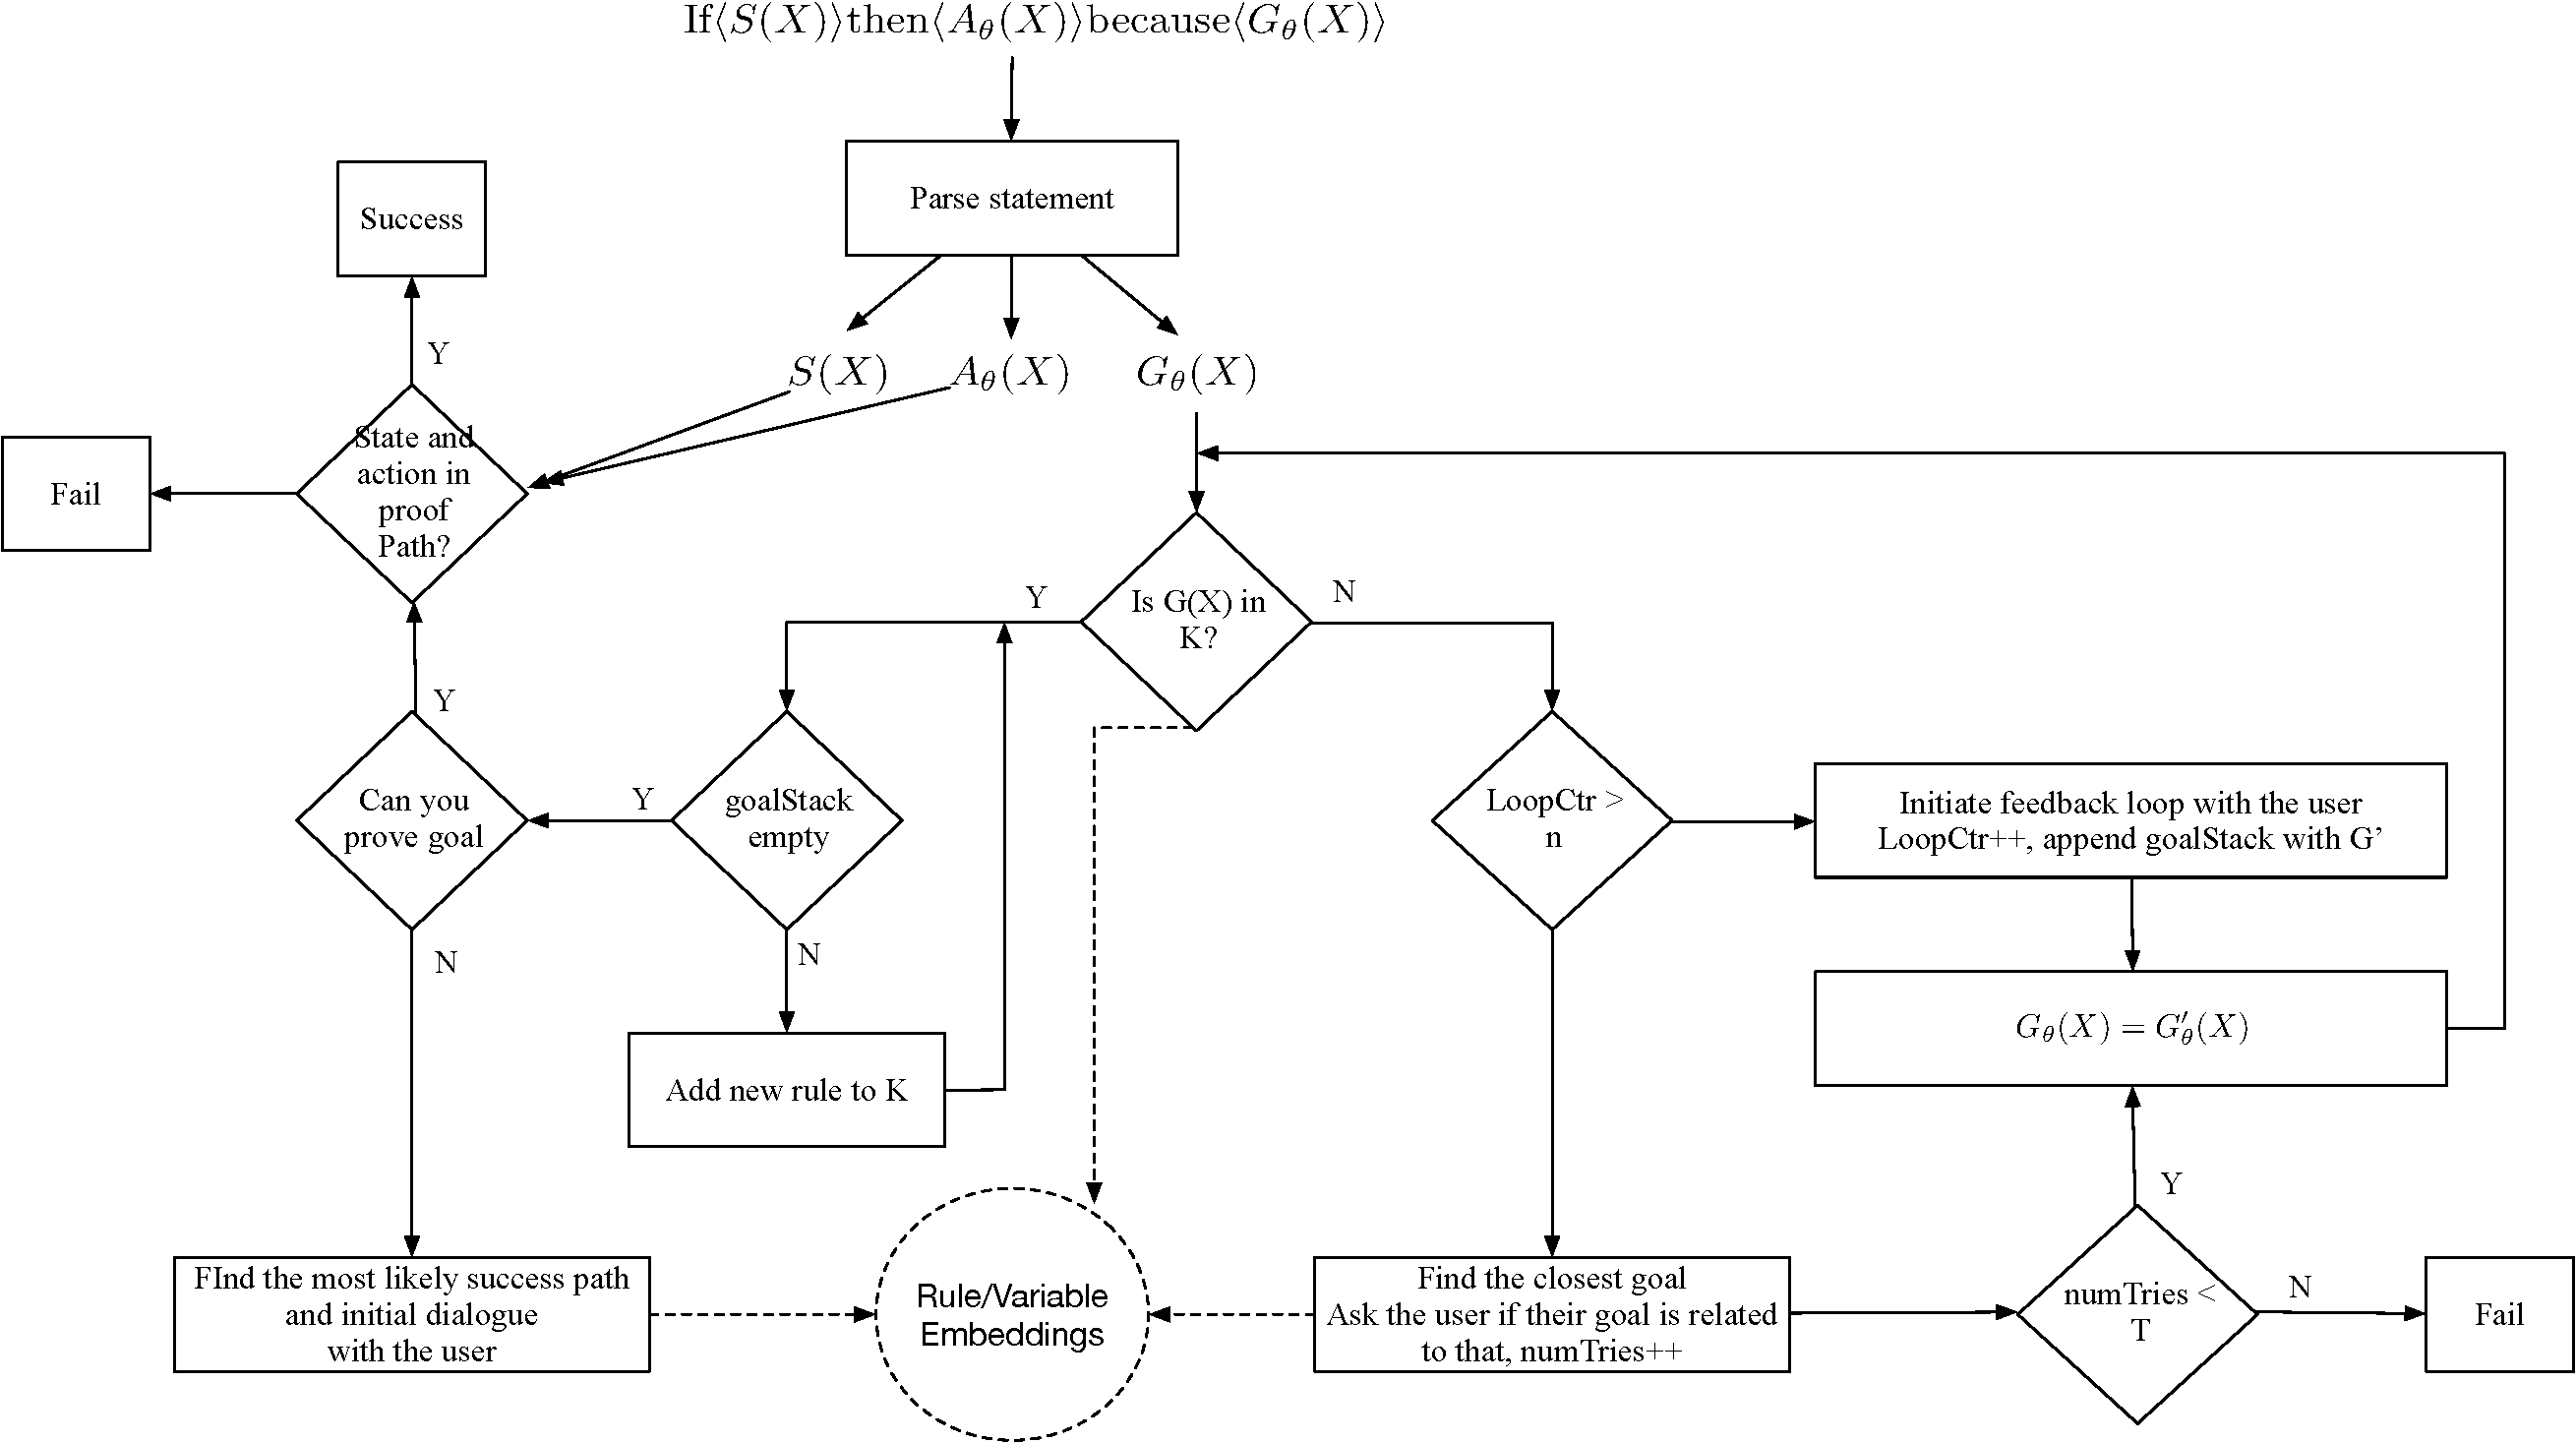
\includegraphics[width=\textwidth]{figs/model.pdf}
    % \caption{Model Architecture \amoscomment{Why 'proposed'? The arrows from S(X) and A(X) make it hard to understand the flow (that is, what happens first, what next). Maybe just remove them or mark it differently (not using arrows).} \facomment{figure is being re-generated}}
    \caption{CORGI's flowchart. The input is an if-then-because command e.g., ``if it snows tonight then wake me up early because I want to get to work on time''. The input is parsed into its logical form representation (for this example, $\state$ = \prologTerm{weather(snow, Precipitation)}). If CORGI succeeds, it outputs a proof tree for the because-clause or \textGoal (parsed into $\goal$=\prologTerm{get(i,work,on$\_$time)}). The output proof tree contains commonsense presumptions for the input statement (Fig \ref{fig:prooftree} shows an example). If the predicate $G$ does not exist in the knowledge base, \KB, (Is $G$ in \KB?), we have missing knowledge and cannot find a proof. Therefore, we extract it from a human in the \emph{user feedback loop}. At the heart of CORGI is a neuro-symbolic theorem prover that learns rule and variable embeddings to perform a proof (Alg.\ref{alg:inference}). $\mathrm{goalStack}$ and the loop variable $i$ are initialized to empty and $0$ respectively, and $n=3$. \emph{italic text} in the figure represents descriptions that are referred to in the main text. }
    \label{fig:model}
    \vspace{-1.5em}
\end{figure*}
% In this paper, we would like to use commonsense background knowledge to extract hidden commonsense presumptions and to engage in a conversation with the user to complete the background knowledge through this interaction. %We assume the user's utterance follows the general format ``if $\langle$\textState $\state \, \text{holds} \rangle$ then $\langle$perform \textAction $\action \rangle$ because $\langle$I want to achieve \textGoal $\goal \rangle$''.
%Our goal is to do commonsense reasoning given a statement of the form ``if ... then ... becauase''. 
% For example, ``If it snows at night then wake me up early because I want to see the snow''.
% For example, ``If the weather is bad tomorrow then remind me to bring my umbrella because I want to stay dry''.